\chapter{Équations de Maxwell}

\minitoc

\section*{Introduction}
\addcontentsline{toc}{section}{Introduction}

En électromagnétisme, on distingue :

\begin{itemize}
    \item le régime statique : \begin{itemize}
        \item électrostatique : théorème de Gauss (1831)
        \item magnétostatique : théorème d'Ampère (1820) \\
    \end{itemize}
    \item le régime variable : \begin{itemize}
        \item induction électromagnétique : loi de Lenz-Faraday (1831-1834).
    \end{itemize}
\end{itemize}

Gauss constate en 1831 l'absence de monopôle magnétique.

En 1865, James Clerk Maxwell réalise l'exploit de synthétiser les résultats expérimentaux en vingt équations scalaires à vingt inconnues écrites à l'aide de quaternions.

Ces équations sont reprises par Oliver Heaviside en 1884 pour aboutir aux quatre équations classiques (deux vectorielles, deux scalaires).

L'électromagnétisme (classique) devient une science aboutie jusqu'à l'arrivée des phénomènes quantiques qui amenèrent l'électrodynamique quantique (Feynman) et la théorie quantique des champs.

\section{Conservation de la charge}

\subsection{Première approche : 1D}

La charge \(q\) est un invariant : elle ne peut être ni créée ni annihilée.

\begin{center}
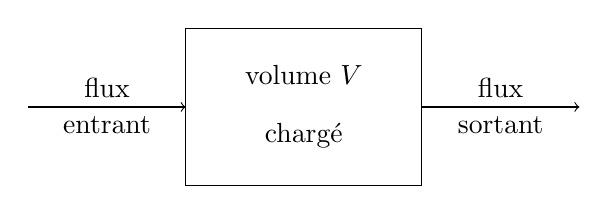
\begin{tikzpicture}
\draw[->] (0,0) -- (2,0) node[above,midway] {flux} node[below,midway] {entrant};
\draw (2,-1) -- (2,1) -- (5,1) node[below=10,midway] {volume \(V\)} -- (5,-1) -- (2,-1) node[above=10,midway] {chargé};
\draw[->] (5,0) -- (7,0) node[above,midway] {flux} node[below,midway] {sortant};
\end{tikzpicture}
\end{center}

La charge au temps \(t\) est égale à la charge initiale plus la charge entrante moins la charge sortante.

À une dimension, on a :

\begin{center}
\begin{tikzpicture}
\draw[->] (0,0) -- (10,0) node[below] {\(x\)};
\draw[->,blue] (0,0) -- (1,0) node[below] {\(\v{u}_x\)};
\draw (3,2) -- (7,2);
\draw (3,5) arc[start angle=90,end angle=270,x radius=1,y radius=1.5];
\draw[dotted] (4,3.5) arc[start angle=0,end angle=90,x radius=1,y radius=1.5];
\draw[dotted] (4,3.5) arc[start angle=0,end angle=-90,x radius=1,y radius=1.5];
\draw (8,3.5) arc[start angle=0,end angle=360,x radius=1,y radius=1.5];
\draw (3,5) -- (7,5);
\draw[dashed] (3,2) -- (3,0) node[below] {\(x\)};
\draw[dashed] (7,2) -- (7,0) node[below] {\(x+\odif{x}\)};
\draw (3,4.9) -- (5,5.5) node[above] {surface \(S\)};
\draw (7,4.9) -- (5,5.5);
\draw[->] (3,3.5) -- (4.5,3.5) node[above right] {\(\v{S}_\entrant\)};
\draw[->,red] (3,3.4) -- (4.5,3.4) node[below right] {\(\v{j}\paren{x,t}\)};
\draw[->] (7,3.5) -- (8.5,3.5) node[above right] {\(\v{S}_\sortant\)};
\draw[->,red] (7,3.4) -- (8.5,3.4) node[below right] {\(\v{j}\paren{x+\odif{x},t}\)};
\end{tikzpicture}
\end{center}

Le cylindre de surface \(S\) et de largeur \(\odif{x}\) est traversé par la densité de courant volumique \(\v{j}\).

\(\v{j}\paren{x,t}\) traverse la surface d'entrée du cylindre.

\(\v{j}\paren{x+\odif{x},t}\) traverse la surface de sortie du cylindre.

\(\rho\paren{x,t}\) : densité volumique de charge du cylindre.

Établissons le bilan des charges dans le cylindre entre \(t\) et \(t+\odif{t}\).

On note \(\fdif{Q_\entrant}\) et \(\fdif{Q_\sortant}\) la charge entrante (respectivement sortante) à travers la surface d'entrée (respectivement de sortie) du cylindre entre \(t\) et \(t+\odif{t}\).

On a \(\fdif{Q_\entrant}=I_\entrant\odif{t}\).

Or \(I_\entrant=\iint\v{j}\scal\odif{\v{S}}=j\paren{x,t}S\).

Donc \(\fdif{Q_\entrant}=j\paren{x,t}S\odif{t}\).

De même, on a \(\fdif{Q_\sortant}=j\paren{x+\odif{x},t}S\odif{t}\).

Donc \[\begin{aligned}
\fdif{Q}&=\fdif{Q_\entrant}-\fdif{Q_\sortant} \\
&=j\paren{x,t}S\odif{t}-j\paren{x+\odif{x},t}S\odif{t} \\
&=\underbrace{\paren{j\paren{x,t}-j\paren{x+\odif{x},t}}}_{-\pdv{j}{x}\odif{x}}S\odif{t}.
\end{aligned}\]

De plus, on a \(Q\paren{t}=\rho\paren{x,t}\odif{\tau}\) avec \(\odif{\tau}=S\odif{x}\) le volume du cylindre.

Pendant la durée \(\odif{t}\), la charge \(Q\paren{t}\) a varié de \[\begin{aligned}
\odif{Q}&=Q\paren{t+\odif{t}}-Q\paren{t} \\
&=\underbrace{\paren{\rho\paren{x,t+\odif{t}}-\rho\paren{x,t}}}_{\pdv{\rho}{t}\odif{t}}\odif{\tau}.
\end{aligned}\]

Or on a \[\begin{aligned}
\odif{Q}&=\fdif{Q} \\
\pdv{\rho}{t}\odif{t}S\odif{x}&=-\pdv{j}{x}\odif{x}S\odif{t} \\
\pdv{\rho}{t}&=-\pdv{j}{x} \\
\color{red}\pdv{\rho}{t}+\pdv{j}{x}&\color{red}=0.\color{black}
\end{aligned}\]

C'est l'équation locale de conservation de la charge à une dimension.

Remarque :

Ici, on a \(\v{j}\paren{x,t}=j\paren{x,t}\v{u}_x\).

On remarque \(\pdv{j}{x}=\div\v{j}\).

Donc l'équation locale de conservation de la charge se réécrit \[\color{red}\div\v{j}+\pdv{\rho}{t}=0.\color{black}\]

\subsection{Généralisation : 3D}

On admet que la formule précédente se généralise à trois dimensions : \[\color{red}\div\v{j}+\pdv{\rho}{t}=0.\color{black}\]

On peut le démontrer avec le théorème d'Ostrogradski-Green.

\section{Les équations de Maxwell}

\subsection{Énoncé}

Équation de Maxwell-Gauss \MG : \[\div\v{E}=\dfrac{\rho}{\epsilon_0}.\]

Équation de Maxwell-Flux ou Maxwell-Thomson \MT : \[\div\v{B}=0.\]

Équation de Maxwell-Faraday \MF : \[\rot\v{E}=-\pdv{\v{B}}{t}.\]

Équation de Maxwell-Ampère \MA : \[\rot\v{B}=\mu_0\v{j}+\mu_0\epsilon_0\pdv{\v{E}}{t}.\]

\subsection{Commentaires}

\begin{itemize}
    \item \MG et \MT sont des équations scalaires. \\
    \item \MF et \MA sont des équations vectorielles. \\
    \item \(\epsilon_0\) est la permittivité diélectrique du vide et \(\mu_0\) est la perméabilité magnétique du vide. On a \[\epsilon_0=\SI{8.85e-12}{\farad\per\metre}\qquad\text{et}\qquad\mu_0=\SI{4\pi e-7}{\henry\per\metre}.\] On verra que \(\mu_0\epsilon_0c^2=1\). \\
    \item \MG, \MT, \MF et \MA sont des équations linéaires : on peut appliquer le principe de superposition. \\
    \item \MG, \MT, \MF et \MA sont des équations locales, elles s'appliquent en un point \(M\), il n'y a pas d'expression intégrale. \\
    \item \MG et \MA relient \(\v{E}\) et \(\v{B}\) à leurs sources (charges et courants). \\
    \item \MF et \MA introduisent un couplage entre \(\v{E}\) et \(\v{B}\) en régime variable ; les champs \(\v{E}\) et \(\v{B}\) sont indissociables. \\
    \item \MG et \MF montrent que pour créer un champ \(\v{E}\), on peut utiliser des charges (\(\rho\)) ou un champ \(\v{B}\) variable (induction électromagnétique). \\
    \item \MA montre que pour créer un champ \(\v{B}\), on peut utiliser un courant (\(\v{j}\)) ou un champ électrique variable. \\
    \item On remarque que \(\v{j}\) est homogène à \(\epsilon_0\pdv{\v{E}}{t}=\v{j}_D\) : courant de déplacement.
\end{itemize}

\subsection{Compatibilité des équations de Maxwell}

On a \MA : \(\rot\v{B}=\mu_0\v{j}+\mu_0\epsilon_0\pdv{\v{E}}{t}\).

On applique \(\div\) : \[\begin{aligned}
\div\paren{\rot\v{B}}&=\div\paren{\mu_0\v{j}+\mu_0\epsilon_0\pdv{\v{E}}{t}} \\
&=0.
\end{aligned}\]

Donc \[\begin{WithArrows}
0&=\mu_0\paren{\div\v{j}+\epsilon_0\pdv{}{t}\div\v{E}} \Arrow{\MG} \\
&=\mu_0\paren{\div\v{j}+\pdv{\rho}{t}}.
\end{WithArrows}\]

Donc \(\div\v{j}+\pdv{\rho}{t}=0\).

Donc les équations de Maxwell sont compatibles avec l'équation locale de conservation de la charge.

\section{Forme intégrale des équations de Maxwell}

\subsection{Théorème de Gauss}

On considère une surface \(S\) fermée définissant le volume \(V\).

Soit \(\phi_{\v{E}}\) le flux de \(\v{E}\) à travers \(S\).

On a \(\phi_{\v{E}}=\oiint_S\v{E}\scal\odif{\v{S}}\).

D'après le théorème d'Ostrogradski-Green, on a \(\oiint_S\v{E}\scal\odif{\v{S}}=\iiint_V\div\v{E}\odif{\tau}\).

Donc \(\phi_{\v{E}}=\iiint_V\div\v{E}\odif{\tau}\).

D'après \MG, on a \(\div\v{E}=\dfrac{\rho}{\epsilon_0}\).

D'où \[\begin{aligned}
\phi_{\v{E}}&=\dfrac{1}{\epsilon_0}\iiint_V\rho\odif{\tau} \\
\color{red}\oiint_S\v{E}\scal\odif{\v{S}}&\color{red}=\dfrac{Q_\inte}{\epsilon_0}.\color{black}
\end{aligned}\]

On a prouvé le théorème de Gauss.

On dit que c'est la forme intégrale de \MG.

\subsection{Conservation du flux magnétique}

Une considère une surface \(S\) définissant le volume \(V\).

On a \[\begin{WithArrows}
\phi_{\v{B}}&=\oiint_S\v{B}\scal\odif{\v{S}} \Arrow{Ostrogradski-Green} \\
&=\iiint_V\div\v{B}\odif{\tau} \Arrow{\MT} \\
&=0.
\end{WithArrows}\]

D'où \[\color{red}\oiint_S\v{B}\scal\odif{\v{S}}=0.\color{black}\]

On a prouvé la conservation du flux magnétique.

On dit que c'est la forme intégrale de \MT.

\subsection{Loi de Lenz-Faraday}

Soit un contour fermé et orienté \(\Gamma\) s'appuyant sur la surface \(\v{S}\) dans une zone traversée par un champ \(\v{B}\).

On calcule \(e\) la circulation de \(\v{E}\) le long de \(\Gamma\) ; c'est la tension (ou force électromotrice) le long de \(\Gamma\). On a vu en MP2I la loi de Lenz-Faraday : \(e=-\odv{\phi}{t}\).

On a \[\begin{WithArrows}
e&=\oint_\Gamma\v{E}\scal\odif{\v{l}} \Arrow{Stokes-Ampère} \\
&=\iint_S\rot\v{E}\scal\odif{\v{S}} \Arrow{\MF} \\
&=\iint_S\paren{-\pdv{\v{B}}{t}}\scal\odif{\v{S}} \\
&=-\pdv{}{t}\iint_S\v{B}\scal\odif{\v{S}} \Arrow{\(\phi=\iint_S\v{B}\scal\odif{\v{S}}\) : flux magnétique} \\
&=-\pdv{\phi}{t} \Arrow{\(\phi\) ne dépend que du temps} \\
&=-\odv{\phi}{t}.
\end{WithArrows}\]

On a prouvé la loi de Lenz-Faraday.

Remarque : comme dans la loi de Lenz-Faraday, dans \MF : \(\rot\v{E}=-\pdv{\v{B}}{t}\), le signe \guillemets{\(-\)} est dû au principe de modération.

\subsection{Théorème d'Ampère généralisé}

Soit un contour fermé et orienté \(\Gamma\) s'appuyant sur la surface \(\v{S}\) dans une zone traversée par un champ \(\v{B}\).

On a \[\begin{WithArrows}
\call{C}&=\oint_\Gamma\v{B}\scal\odif{\v{l}} \Arrow{Stokes-Ampère} \\
&=\iint_S\rot\v{B}\scal\odif{\v{S}} \Arrow{\MA} \\
&=\iint_S\mu_0\v{j}\scal\odif{\v{S}}+\iint_S\mu_0\epsilon_0\pdv{\v{E}}{t}\scal\odif{\v{S}} \\
&=\mu_0\iint_S\v{j}\scal\odif{\v{S}}+\mu_0\epsilon_0\pdv{}{t}\iint_S\v{E}\scal\odif{\v{S}} \\
&\color{red}=\mu_0I_\enl+\mu_0\epsilon_0\pdv{}{t}\iint_S\v{E}\scal\odif{\v{S}}.
\end{WithArrows}\]

C'est le théorème d'Ampère généralisé.

Remarque : en statique, on a \(\pdv{}{t}=0\) donc on retrouve le théorème d'Ampère \(\call{C}=\mu_0I_\enl\).

\subsection{Bilan}

\begin{center}
\begin{Tabular}{c|c}
\thead{Loi locale} & \thead{Loi intégrale} \\
\hline \\
\MG : \(\div\v{E}=\dfrac{\rho}{\epsilon_0}\) & Théorème de Gauss : \(\oiint\v{E}\scal\odif{\v{S}}=\dfrac{Q_\inte}{\epsilon_0}\) \\\\
\MT : \(\div\v{B}=0\) & Conservation du flux magnétique : \(\oiint\v{B}\scal\odif{\v{S}}=0\) \\\\
\MF : \(\rot\v{E}=-\pdv{\v{B}}{t}\) & Loi de Lenz-Faraday : \(e=\oint\v{E}\scal\odif{\v{l}}=-\odv{\phi}{t}\) \\\\
\MA : \(\rot\v{B}=\mu_0\v{j}+\mu_0\epsilon_0\pdv{\v{E}}{t}\) & \makecell{Théorème d'Ampère généralisé : \\ \(\call{C}=\oint\v{B}\scal\odif{\v{l}}=\mu_0I_\enl+\mu_0\epsilon_0\pdv{}{t}\iint\v{E}\scal\odif{\v{S}}\)}
\end{Tabular}
\end{center}

\note{Chapitre incomplet : progression du 20/11}
